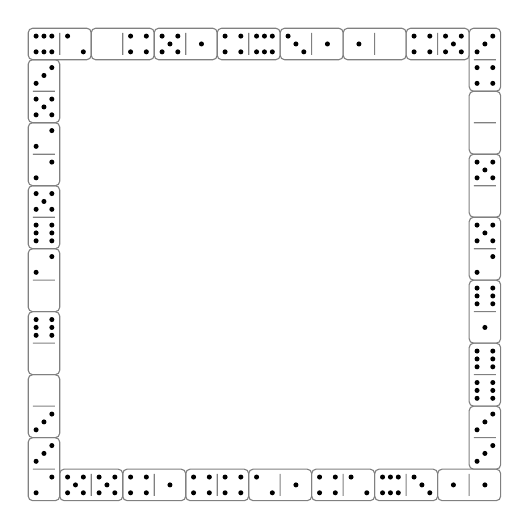
\begin{tikzpicture}[scale=.4]
\def\one{+(0.00,0.00) circle [radius=0.08]}
\def\two{+(-.25, .25) circle [radius=0.08]
	 +( .25,-.25) circle [radius=0.08]}
\def\thr{+(-.25, .25) circle [radius=0.08]
	 +(0.00,0.00) circle [radius=0.08]
	 +( .25,-.25) circle [radius=0.08]}
\def\fou{+(-.25,-.25) circle [radius=0.08]
	 +(-.25, .25) circle [radius=0.08]
	 +( .25,-.25) circle [radius=0.08]
	 +( .25, .25) circle [radius=0.08]}
\def\fiv{+(-.25,-.25) circle [radius=0.08]
	 +(-.25, .25) circle [radius=0.08]
	 +(0.00,0.00) circle [radius=0.08]
	 +( .25,-.25) circle [radius=0.08]
	 +( .25, .25) circle [radius=0.08]}
\def\six{+(-.25,-.25) circle [radius=0.08]
	 +(-.25, .25) circle [radius=0.08]
	 +(0.00,-.25) circle [radius=0.08]
	 +(0.00, .25) circle [radius=0.08]
	 +( .25,-.25) circle [radius=0.08]
	 +( .25, .25) circle [radius=0.08]}
\def\domino{
  [rounded corners=1.6pt]+(-1,-.5) rectangle +(1,.5)
  [gray,thin]+(0,.35) -- +(0,-.35)
}
\draw (-6.5, 7.0) \domino;
\fill (-6.5, 7.0) ++(-0.5,0) \six;
\fill (-6.5, 7.0) ++( 0.5,0) \two;
\draw (-4.5, 7.0) \domino;
%\fill (-4.5, 7.0) ++(-0.5,0) \six;
\fill (-4.5, 7.0) ++( 0.5,0) \fou;
\draw (-2.5, 7.0) \domino;
\fill (-2.5, 7.0) ++(-0.5,0) \fiv;
\fill (-2.5, 7.0) ++( 0.5,0) \one;
\draw (-0.5, 7.0) \domino;
\fill (-0.5, 7.0) ++(-0.5,0) \fou;
\fill (-0.5, 7.0) ++( 0.5,0) \six;
\draw ( 1.5, 7.0) \domino;
\fill ( 1.5, 7.0) ++(-0.5,0) \thr;
\fill ( 1.5, 7.0) ++( 0.5,0) \one;
\draw ( 3.5, 7.0) \domino;
\fill ( 3.5, 7.0) ++(-0.5,0) \one;
%\fill ( 3.5, 7.0) ++( 0.5,0) \six;
\draw ( 5.5, 7.0) \domino;
\fill ( 5.5, 7.0) ++(-0.5,0) \fou;
\fill ( 5.5, 7.0) ++( 0.5,0) \fiv;
\begin{scope}[rotate=90]
  \draw (-6.5, 7.0) \domino;
  \fill (-6.5, 7.0) ++(-0.5,0) \two;
  \fill (-6.5, 7.0) ++( 0.5,0) \thr;
  \draw (-4.5, 7.0) \domino;
  \fill (-4.5, 7.0) ++(-0.5,0) \thr;
%  \fill (-4.5, 7.0) ++( 0.5,0) \six;
  \draw (-2.5, 7.0) \domino;
%  \fill (-2.5, 7.0) ++(-0.5,0) \six;
  \fill (-2.5, 7.0) ++( 0.5,0) \six;
  \draw (-0.5, 7.0) \domino;
%  \fill (-0.5, 7.0) ++(-0.5,0) \six;
  \fill (-0.5, 7.0) ++( 0.5,0) \two;
  \draw ( 1.5, 7.0) \domino;
  \fill ( 1.5, 7.0) ++(-0.5,0) \six;
  \fill ( 1.5, 7.0) ++( 0.5,0) \fiv;
  \draw ( 3.5, 7.0) \domino;
  \fill ( 3.5, 7.0) ++(-0.5,0) \two;
  \fill ( 3.5, 7.0) ++( 0.5,0) \two;
  \draw ( 5.5, 7.0) \domino;
  \fill ( 5.5, 7.0) ++(-0.5,0) \fiv;
  \fill ( 5.5, 7.0) ++( 0.5,0) \thr;
\end{scope}
\begin{scope}[rotate=180]
  \draw (-6.5, 7.0) \domino;
  \fill (-6.5, 7.0) ++(-0.5,0) \one;
  \fill (-6.5, 7.0) ++( 0.5,0) \one;
  \draw (-4.5, 7.0) \domino;
  \fill (-4.5, 7.0) ++(-0.5,0) \thr;
  \fill (-4.5, 7.0) ++( 0.5,0) \six;
  \draw (-2.5, 7.0) \domino;
  \fill (-2.5, 7.0) ++(-0.5,0) \two;
  \fill (-2.5, 7.0) ++( 0.5,0) \fou;
  \draw (-0.5, 7.0) \domino;
  \fill (-0.5, 7.0) ++(-0.5,0) \one;
  \fill (-0.5, 7.0) ++( 0.5,0) \two;
  \draw ( 1.5, 7.0) \domino;
  \fill ( 1.5, 7.0) ++(-0.5,0) \fou;
  \fill ( 1.5, 7.0) ++( 0.5,0) \fou;
  \draw ( 3.5, 7.0) \domino;
  \fill ( 3.5, 7.0) ++(-0.5,0) \one;
  \fill ( 3.5, 7.0) ++( 0.5,0) \fou;
  \draw ( 5.5, 7.0) \domino;
  \fill ( 5.5, 7.0) ++(-0.5,0) \fiv;
  \fill ( 5.5, 7.0) ++( 0.5,0) \fiv;
\end{scope}
\begin{scope}[rotate=270]
  \draw (-6.5, 7.0) \domino;
  \fill (-6.5, 7.0) ++(-0.5,0) \thr;
  \fill (-6.5, 7.0) ++( 0.5,0) \fou;
  \draw (-4.5, 7.0) \domino;
%  \fill (-4.5, 7.0) ++(-0.5,0) \fou;
%  \fill (-4.5, 7.0) ++( 0.5,0) \two;
  \draw (-2.5, 7.0) \domino;
  \fill (-2.5, 7.0) ++(-0.5,0) \fiv;
%  \fill (-2.5, 7.0) ++( 0.5,0) \six;
  \draw (-0.5, 7.0) \domino;
  \fill (-0.5, 7.0) ++(-0.5,0) \fiv;
  \fill (-0.5, 7.0) ++( 0.5,0) \two;
  \draw ( 1.5, 7.0) \domino;
  \fill ( 1.5, 7.0) ++(-0.5,0) \six;
  \fill ( 1.5, 7.0) ++( 0.5,0) \one;
  \draw ( 3.5, 7.0) \domino;
  \fill ( 3.5, 7.0) ++(-0.5,0) \six;
  \fill ( 3.5, 7.0) ++( 0.5,0) \six;
  \draw ( 5.5, 7.0) \domino;
  \fill ( 5.5, 7.0) ++(-0.5,0) \thr;
  \fill ( 5.5, 7.0) ++( 0.5,0) \thr;
\end{scope}
\end{tikzpicture}
